\chapter{Practice: Publishing data in Xively}

This lab practice is derived from Xively's documentation. You may find the original post at \emph{\color{blue}{\href{https://xively.com/dev/tutorials/curl}{Xively's tutorials webpage}}}.

Create a user in \emph{\color{blue}{\href{http://xively.com}{Xively.com}}} .
You will receive an email with a pointer to create an API-Key.
%Create this key as you will need it to interact with Xively.

Use the API Key you obtained in the previous step and added to the \texttt{--header} field in Listing~\ref{code:create-feed}. This code effectively creates a feed for your data. Notice the terminal's output in Fig.~\ref{fig:create-feed} and you will observe a feed ID (the last number in the \emph{Location} line near the end).

\begin{lstlisting} [caption = {Command to create a feed}, language = sh, label = {code:create-feed}, numbers = left, escapeinside={@}{@}]
curl --request POST \
     --data '{"title":"My feed", "version":"1.0.0"}' \
     --header "X-ApiKey: <YOUR_API_KEY_HERE>" \
     --verbose \
     http://api.xively.com/v2/feeds

\end{lstlisting}

Next edit a JSON file (name it, for example, \texttt{xively.json}) with the contents detailed in Listing \ref{code:data-json}. This file mimics data gathered from your sensors, and is going to be uploaded to the feed you created with the help of Listing~\ref{code:create-feed}.

\begin{figure}[htbp]
  \centering
  \includegraphics[width=0.9\linewidth]{figures/create-feed.eps}
  \caption{Creating a feed in Xively using curl}
  \label{fig:create-feed}
\end{figure}

Create a JSON file with some dummy data to update your Xively feed as shown in Listing \ref{code:data-json}.

\begin{lstlisting} [caption = {JSON file with data to be uploaded to Xively}, language = sh, label = {code:data-json}, numbers = left, escapeinside={@}{@}]
{
  "version":"1.0.0",
  "datastreams":[
      {"id":"0", "current_value":"100"},
      {"id":"two", "current_value":"500"},
      {"id":"3.0", "current_value":"300"}
  ]
}
\end{lstlisting}

And now you can update your Xively feed using the curl command.\\

\begin{lstlisting} [caption = {Command to upload data to a feed}, language = sh, label = {code:uploading}, numbers = left, escapeinside={*}{*}]
curl --request PUT \
     --data-binary @xively.json \
     --header "X-ApiKey: <YOUR-API-KEY-HERE>" \
     --verbose \
     http://api.xively.com/v2/feeds/<YOUR-FEED-ID>
\end{lstlisting}

And if we look on Xively's web interface, we should be able to see some beautiful plots as in Fig. \ref{fig:plots}

\begin{figure}[htbp]
  \centering
  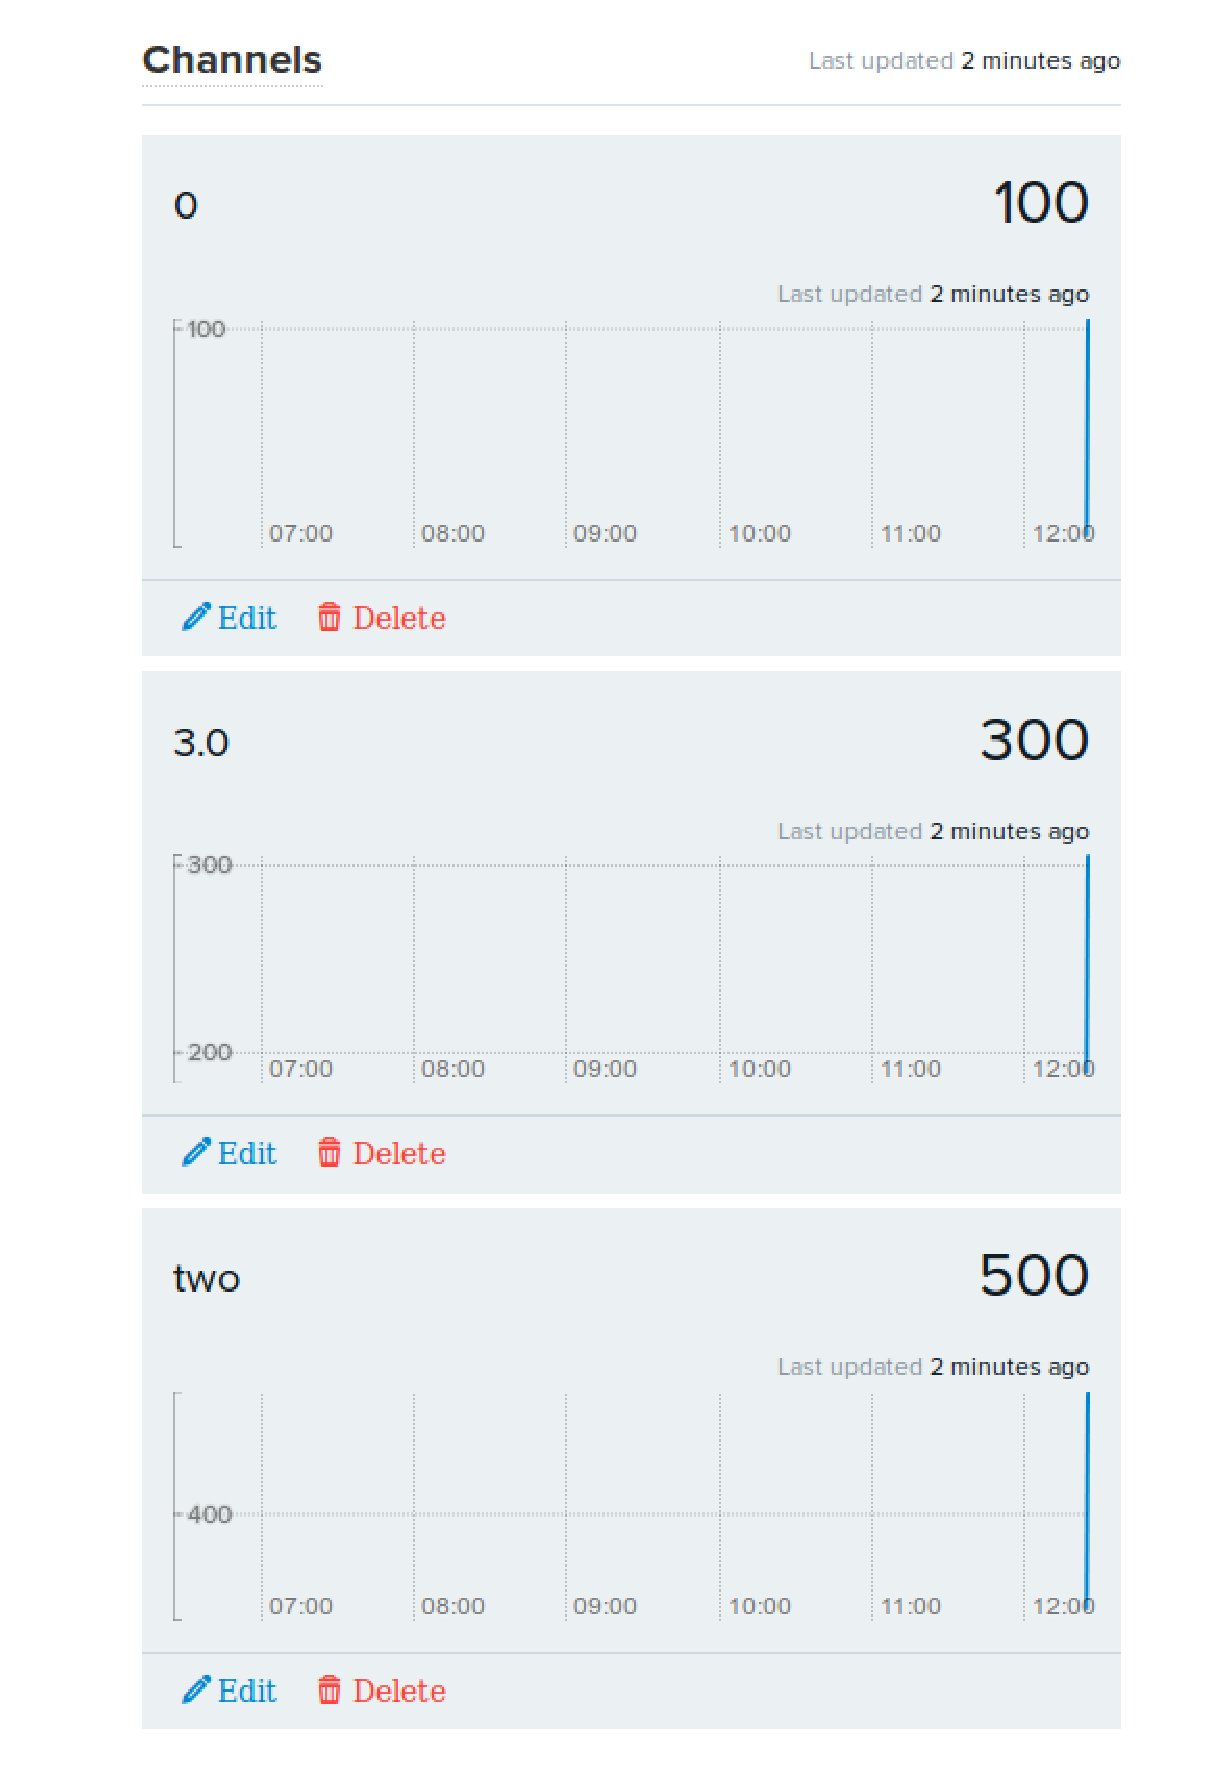
\includegraphics[width=0.6\linewidth]{figures/exportToXively.eps}
  \caption{Plotting data}
  \label{fig:plots}
\end{figure}

You can also read data from the command line as exemplified in Fig. \ref{fig:reading-cosm}.

\begin{figure}[htbp]
  \centering
  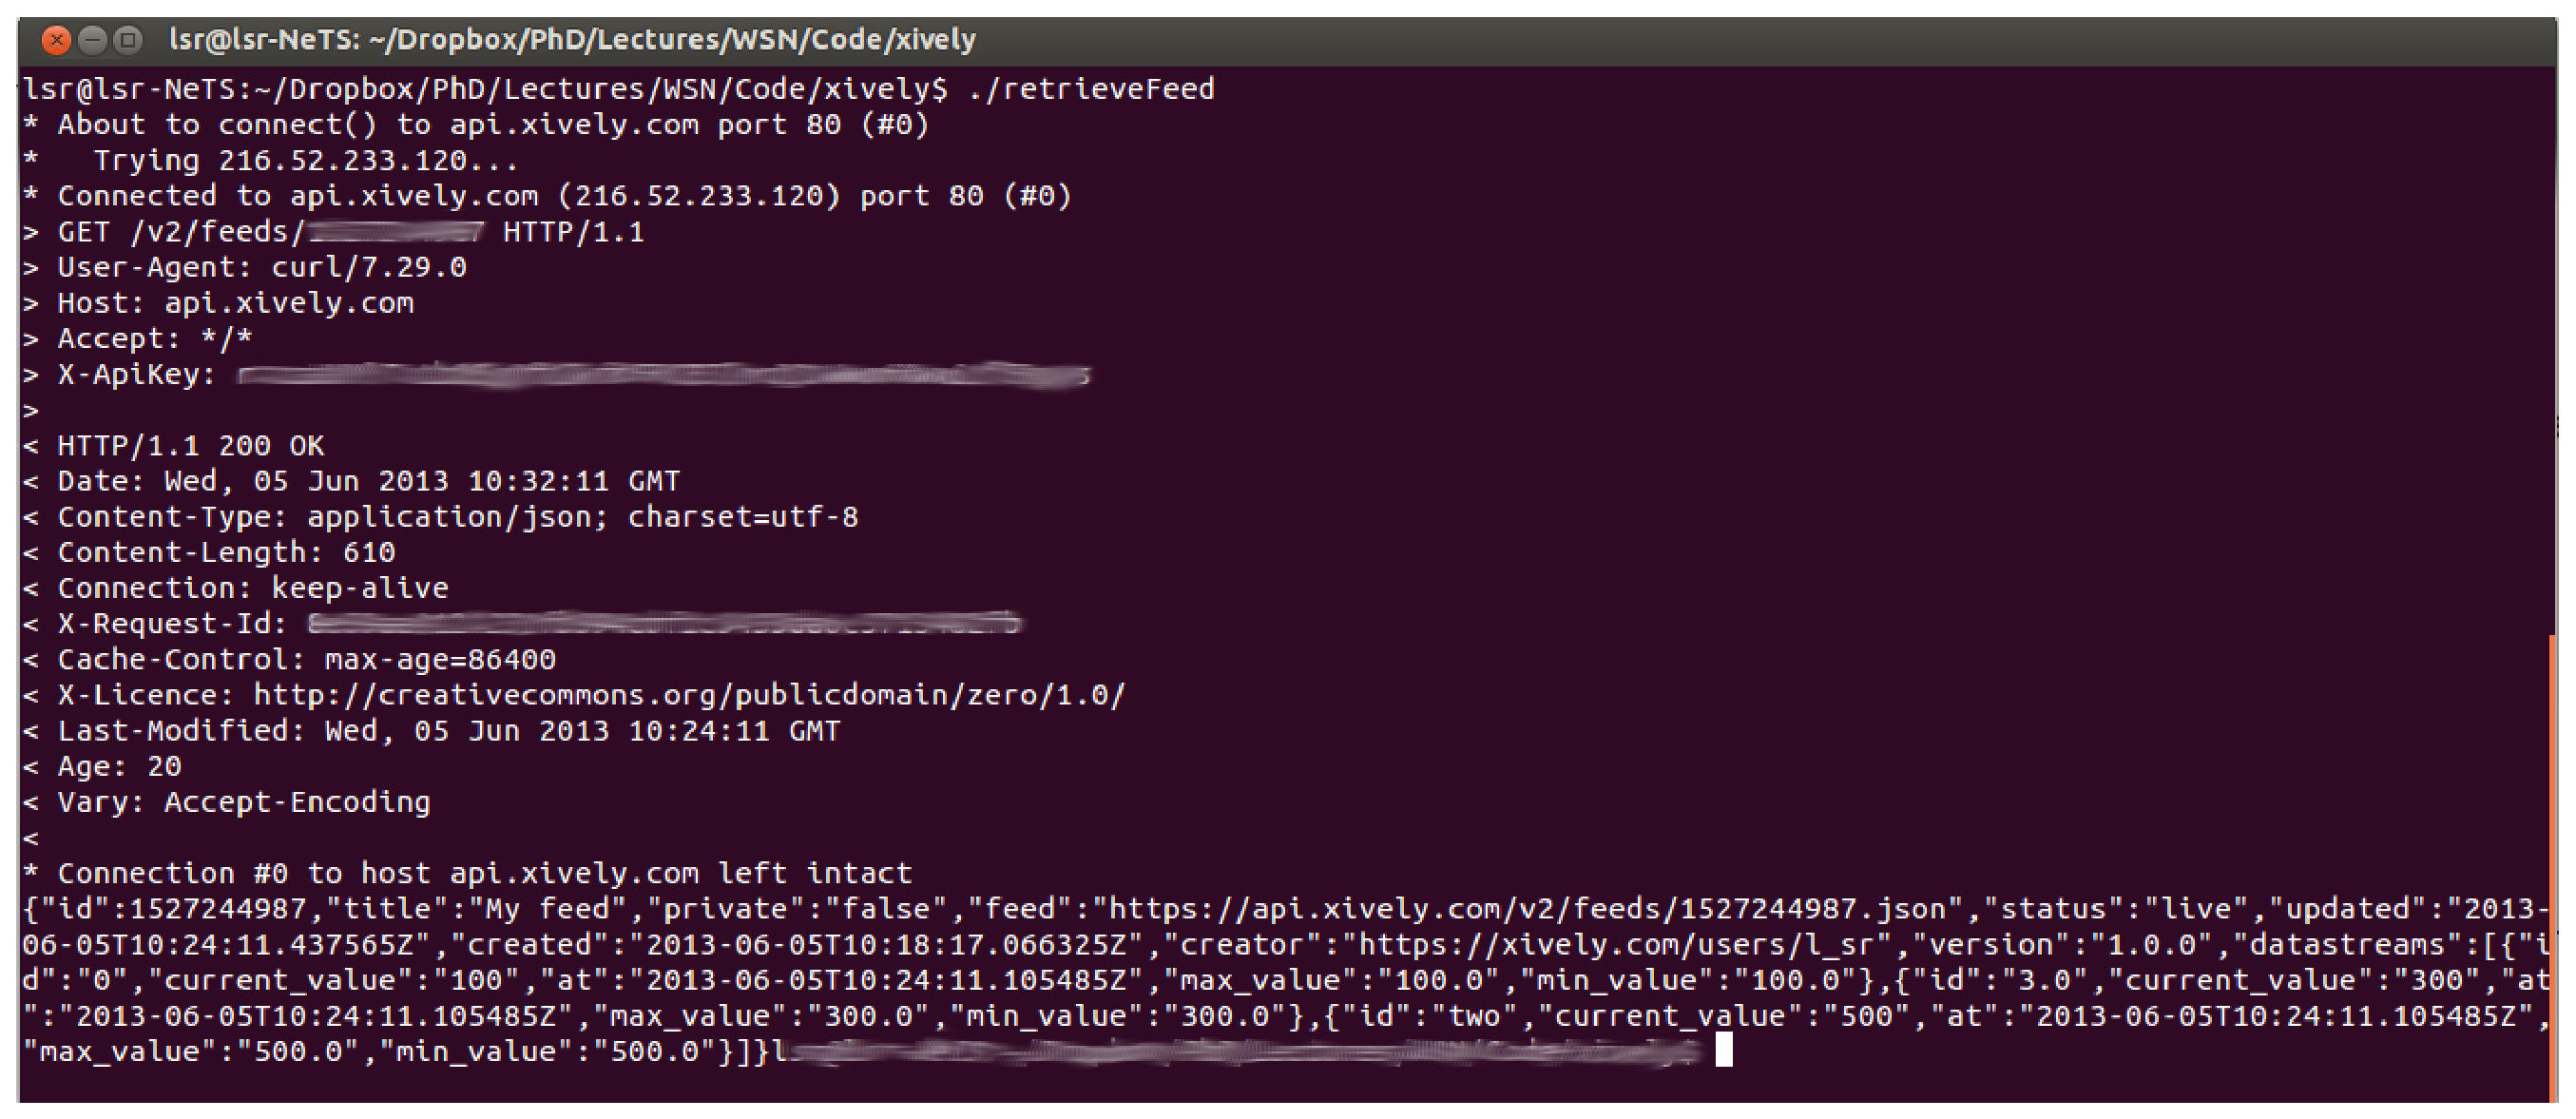
\includegraphics[width=0.9\linewidth]{figures/retrieveXively.eps}
  \caption{Reading a Xively feed from the command line}
  \label{fig:reading-cosm}
\end{figure}

The next step is to gather information from an XBee and publish it to Xively.
Use the code detailed in Listing \ref{code:XBee2Xively} as a reference. We will use the same setup as in Figure~\ref{fig:sunset_sensor} but instead of connecting the coordinator to the Arduino, it will be connected to a host computer through an USB cable.

\begin{lstlisting} [caption = {Command to upload data to a Xively feed}, language = python, label = {code:XBee2Xively}, numbers = left, escapeinside={*}{*}]
# Derived from code by Alejandro Andreu
import commands
import json
import serial
import time
from serial import SerialException
from xbee import ZigBee

print 'Asynchronously printing data from remote XBee'

serial_port = serial.Serial('/dev/ttyUSB0', 9600)

def print_data(data):
    """
    This method is called whenever data is received.
    Its only argument is the data within the frame.
    """
    print data['samples'][0].keys()[0]

    # Create a JSON file and fill it with the received samples
    json_data = {}
    json_data['version'] = '0.2'
    json_data['datastreams'] = ()
    json_data['datastreams'] = json_data['datastreams'] + ({'id': data['samples'][0].keys()[0], 'current_value': str(data['samples'][0].values()[0])},)
    # Add more datastreams if needed
    with open('Xbee2Xively.json', mode='w') as f:
        json.dump(json_data, f, indent = 4)
    # Upload information to Xively. Use your own Api Key and feed identifier
    commands.getstatusoutput('curl --request PUT --data-binary @Xbee2Xively.json --header "X-ApiKey: <YOUR API KEY>" --verbose http://api.xively.com/v2/feeds/<YOUR FEED ID>')

zigbee = ZigBee(serial_port, callback = print_data)

time.sleep(<AS MANY SECONDS AS YOU WANT TO GATHER DATA>)

zigbee.halt();
serial_port.close()
\end{lstlisting}

Now you can pursue more challenging goals.
For example:
\begin{itemize}
\item Gather information from multiple sensors in a node.
\item Gather information from multiple nodes.
\item Transform the measures of the temperature sensor to Celsius degrees.
\end{itemize}

